\documentclass[a4paper,10pt]{article}

\usepackage[ansinew]{inputenc}
\usepackage[spanish]{babel}
\usepackage{graphicx}
\usepackage{listings}
\usepackage{appendix}
\usepackage{pdfpages}
\usepackage{fancyhdr}
\usepackage{paralist}
\pagestyle{fancy}

\begin{document}

\lhead{\fancyplain{}{Organizaci\'on de computadoras 66.20 - Turno Martes}}
\rhead{\fancyplain{}{Trabajo Pr\'actico 1A}}

\setcounter{page}{2}

\newpage
\thispagestyle{empty}
\tableofcontents

\newpage
\section{Introducci\'on}
   En el presente trabajo pr\'actico se busc\'o  familiarizarse con el conjunto de instrucciones MIPS y el concepto de ABI. Para ello se implementaron dos programas completamente en assembly MIPS, que permiten convertir informaci\'on exclusivamente por stdin y stdout, para transformarla de UNIX a DOS y viceversa. Es decir, siguiendo la l\'inea de trabajo de los pr\'acticos anteriores, buscamos generar dos binarios diferentes en vez de un \'unico programa que resuelva ambos problemas.

\section{Resoluci\'on del problema}
  Lo primero que se realiz\'o para cada funci\'on del programa, fue realizar su Stack Frame correspondiente.
  Para ellos se tuvo en cuentas los siguientes puntos: 
  \begin{itemize}
    \item El Stack Frame se compone de \'areas de un tama\~no m\'ultiplo de 8 bytes, alineadas a 8 bytes.
    \item Los registros en un \'area se almacenan de abajo hacia arriba, en orden seg\'un el n\'umero de registro.
    \item Las \'areas son, en orden de aparici\'on (de arriba hacia abajo en memoria):
      \begin{enumerate}
	  \item General Register Save Area[SRA] (obligatoria 3). Registros salvados:
	    \begin{itemize}
	      \item Siempre: \$fp, gp;
	      \item Cuando la funci\'on es non-leaf: ra;
	      \item Si es necesario: el resto de los general purpose callee-saved regs.
	    \end{itemize}
	  \item Floating-Point Registers Save Area: f20 a f30 si es necesario.
	  \item Local and Temporary Variables Area[LTA].
	  \item Unspecified Area[UA]. (obligatoria, aparece siempre, no se almacena nada en ella y es de 8 bytes).
	  \item Argument Building Area[ABA].
	    \begin{itemize}
	      \item Se crea cuando la funci\'on es non-leaf;
	      \item Al menos es de 16 bytes, a\'un cuando los argumentos del callee requieren menos.
	      \item Cuando los cuatro primeros argumentos son enteros o punteros, se pasan en a0 a a3, y el resto se guarda en esta \'area a partir de los primeros 16 bytes.
	      \item Los argumentos pasados en a0 a a3 son almacenados en esta \'area por el callee siempre
	    \end{itemize}
      \end{enumerate}
  \end{itemize}
  
  A continuaci\'on se muestras los Stacks Frames de cada funci\'on de los programas.

  \subsection{Main}
    \subsubsection{Stack frame}
    Los stacks frame de ambos programas son iguales, encontramos tres \'areas:
    \begin{itemize}
      \item SRA: Los registros salvados son: \$fp, gp y ra(por ser una funci\'on non-leaf). Es un \'area de 	      tama\~no de 16 bytes, como debe ser m\'ultiplo de 8 bytes se agrega align[4].
      \item UA: Obligatoria, de 8 bytes.
      \item ABA: Al ser una funci\'on non leaf necesita tres argumentos, por lo que el tama\~no es de 16 	      bytes(con align[4] para ser m\'ultiplo de 8 bytes). 
    \end{itemize}
    La diferencia se presenta en el contenido que poseen los registros FIN\_LINEA y FIN\_LINEA\_NUEVA, presentes en el \'area ABA. En el caso de unix2dos, FIN\_LINEA es \textbackslash n y FIN\_LINEA\_NUEVA \textbackslash r\textbackslash n.
      \begin{center}
	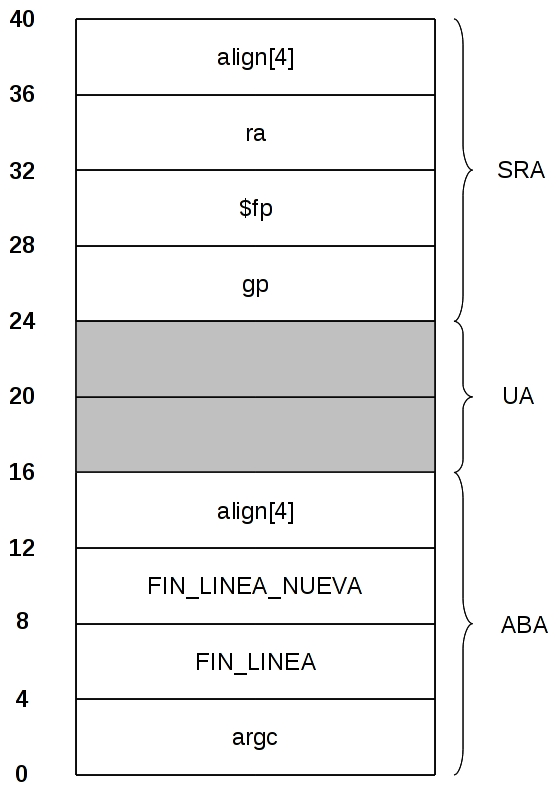
\includegraphics[width=8cm, height=10cm]{DibujosStackFrame/stack-main.jpg}
      \end{center}

  \subsection{Funci\'on conversor unix2dos}
  El stack frame del conversor de unix2dos tiene cuatro \'areas:
      \begin{itemize}
      \item SRA: Los registros salvados son: \$fp, gp y ra. Es un \'area de tama\~no de 16 bytes.
      \item LTA: Se utiliza tres variables locales, dos de 4 bytes(int) y una de 1 byte(char). Es un \'area de tama\~no de 16 bytes
      \item UA: Obligatoria, de 8 bytes.
      \item ABA: Al ser una funci\'on non leaf necesita tres argumentos como m\'aximo, por lo que el tama\~no es de 16 bytes. 
    \end{itemize}
    \subsubsection{Stack frame unix2dos}
      \begin{center}
	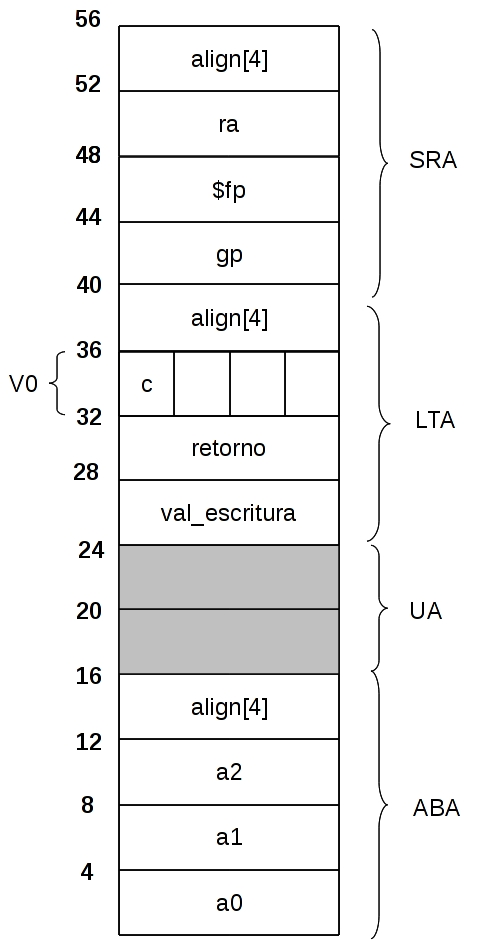
\includegraphics[width=10cm, height=15cm]{DibujosStackFrame/stack-conversor-unix2dos.jpg}
      \end{center}

  \subsection{Funci\'on conversor dos2unix}
  El stack frame del conversor de dos2unix tiene cuatro \'areas:
      \begin{itemize}
      \item SRA: Los registros salvados son: \$fp, gp y ra. Es un \'area de tama\~no de 16 bytes.
      \item LTA: Se utiliza tres variables locales, dos de 4 bytes(int) y dos de 1 byte(char). Es un \'area de tama\~no de 16 bytes
      \item UA: Obligatoria, de 8 bytes.
      \item ABA: Al ser una funci\'on non leaf necesita tres argumentos como m\'aximo, por lo que el tama\~no es de 16 bytes. 
    \end{itemize}
    \subsubsection{Stack frame dos2unix}
      \begin{center}
	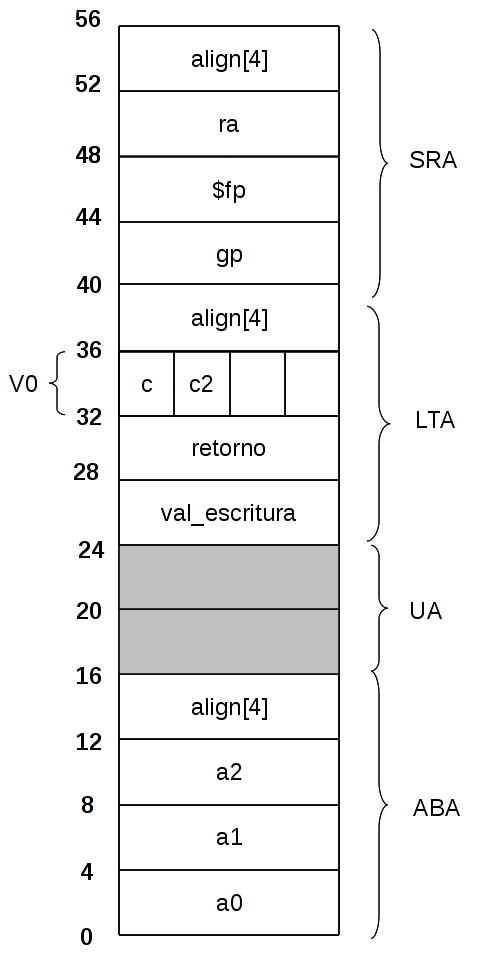
\includegraphics[width=10cm, height=15cm]{DibujosStackFrame/stack-conversor-dos2unix.jpg}
      \end{center}

\section{Preparando el ambiente para NetBSD}
  Para probar el trabajo pr\'actico, lo primero que se debe realizar es enviar el c\'odigo assembly al entorno
  del NetBSD. Se considera que el NetBSD se encuentra corriendo y que se ha creado el loopback necesario. Para ello, se deben realizar los siguientes pasos:
  \begin{enumerate}
   \item Abrir una consola e ingresar en modo root.
   \item Copiar la carpeta ``Codigo`` del cd, a la carpeta del usuario gxemul:
    \newline 
      {\bf hostOS\# cp -r \textbackslash Unidad\_de\_CD\textbackslash Codigo \textbackslash home\textbackslash gxemul}
   \item Conectar con el NetBSD a trav\'es de un t\'unel, se debe ingresar el password correspondiente al 
	 usuario root del NetBSD:
    \newline
      {\bf hostOS\# ssh -p 2222 root@127.0.0.1}
   \item Crear una carpeta para el Tp1, opcional se utiliza para una mejor organizaci\'on:
    \newline 
    {\bf guestOS\# mkdir Tp1}
   \item Copiar la carpeta ''Codigo`` a la carpeta Tp1 del NetBSD, se debe ingresar el password correspondiente al
         usuario gxemul del sistema operativo host:
   \newline
    {\bf guestOS\# scp -r gxemul@172.20.0.1:\textbackslash home\textbackslash gxemul\textbackslash Codigo \newline Tp1\textbackslash }
  \end{enumerate} 

\section{Compilando en NetBSD}
  Para poder compilar desde NetBSD, primero abrir la ubicaci\'on Codigo/Assembly y luego ejecutar:
  \newline
  {\bf guestOS\# cc -o unix2dos unix2dos.S} \newline
  {\bf guestOS\# cc -o dos2unix dos2unix.S}
  \newline
  En ambos casos, se decidi\'o utilizar como nombre archivo de salida (opci\'on -o) el mismo del archivo 
  del c\'odigo assembly.

\section{Ejecutando los programas en NetBSD}
  Para ejecutar el programa, el comando a utilizar es:
  \newline
  {\bf ./[nombre de ejecutable]}
  \newline
  A diferencia del pr\'actico 0, en este solo se utiliza como entrada stdin, y como salida stdout.

\section{Casos de prueba}
  Para la prueba de los programas se utilizaron los mismos archivos del pr\'actico anterior y se agregaron los casos de prueba que
  se solicitan en el enunciado. En todas las pruebas se redirecciona la salida a un archivo para mostrar el contenido con el comando 'hexdump'.
    \subsection{Prueba 1}
    Invocaci\'on del programa con el archivo testdos.txt:
    \begin{itemize}
      \item En la figura se muestra la ejecuci\'on primero del programa unix2dos y se redirecciona la salida al 	archivo 'salida\_dos.txt'. Luego el contenido del archivo de salida se lo pasa por stdin al programa dos2unix, dando como salida un resultado identico al archivo original 'testdos.txt' como era de esperarse.
      \newline
       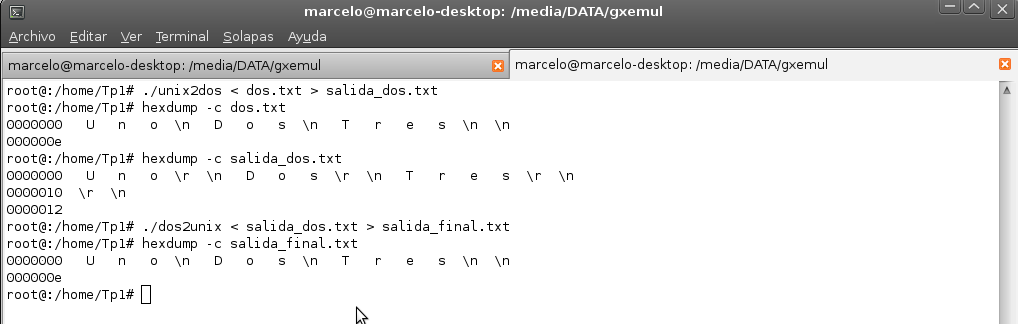
\includegraphics[width=10cm, viewport=0 0 1018 324]{Imagenes/testdos.png}       
    \end{itemize}

    \subsection{Prueba 2}
    Invocaci\'on del programa unix2dos con el archivo testLinux.txt:
    \begin{itemize}
     \item Como se puede ver en las im\'agenes, la unica variaci\'on entre la entrada y la salida son los caracteres de fin de l\'inea.	
     \newline
      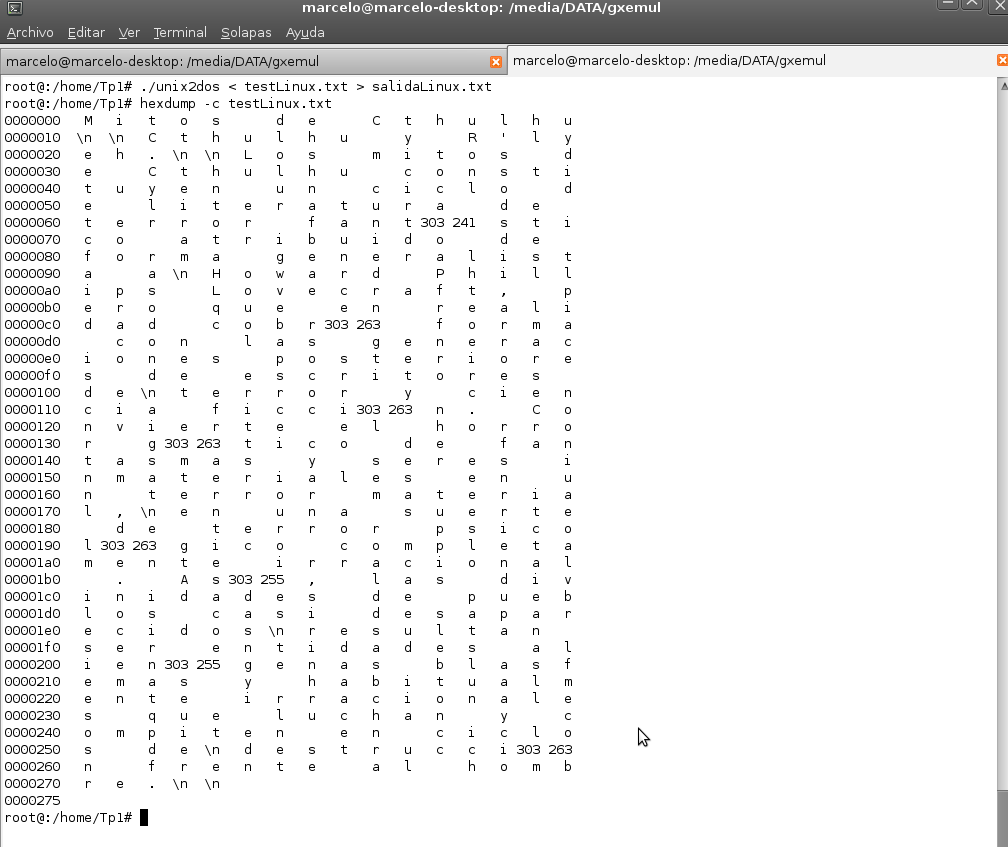
\includegraphics[width=10cm, viewport=0 0 1008 847]{Imagenes/testLinux.png}
     \newline
      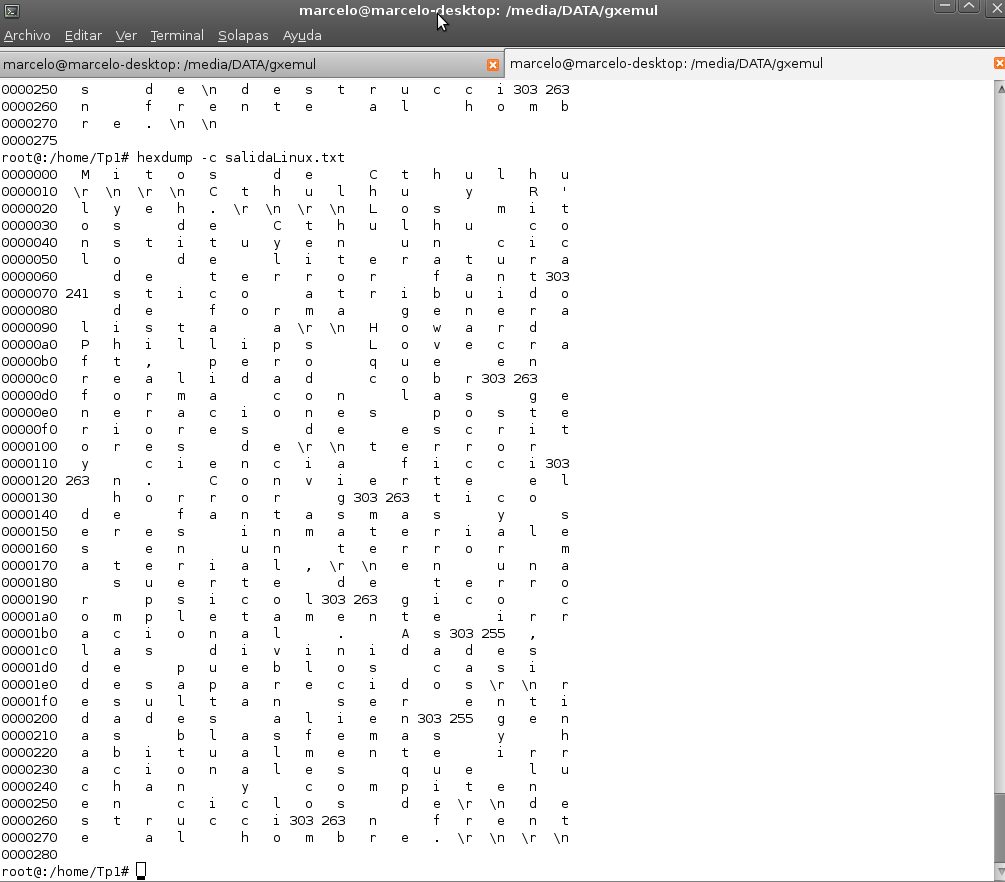
\includegraphics[width=10cm, viewport=0 0 1005 882]{Imagenes/salidaLinux.png}
    \end{itemize}

    \subsection{Prueba 3}
    Invocaci\'on del programa dos2unix con el archivo testWindows.txt:
    \begin{itemize}
     \item El contenido del archivo testWindows.txt es el mismo que testLinux.txt exceptuando al caracter fin de l\'inea.En este caso se puede ver que el resultado coincide con el contenido del archivo testLinux.txt, mencionado en la Prueba 2.
     \newline
      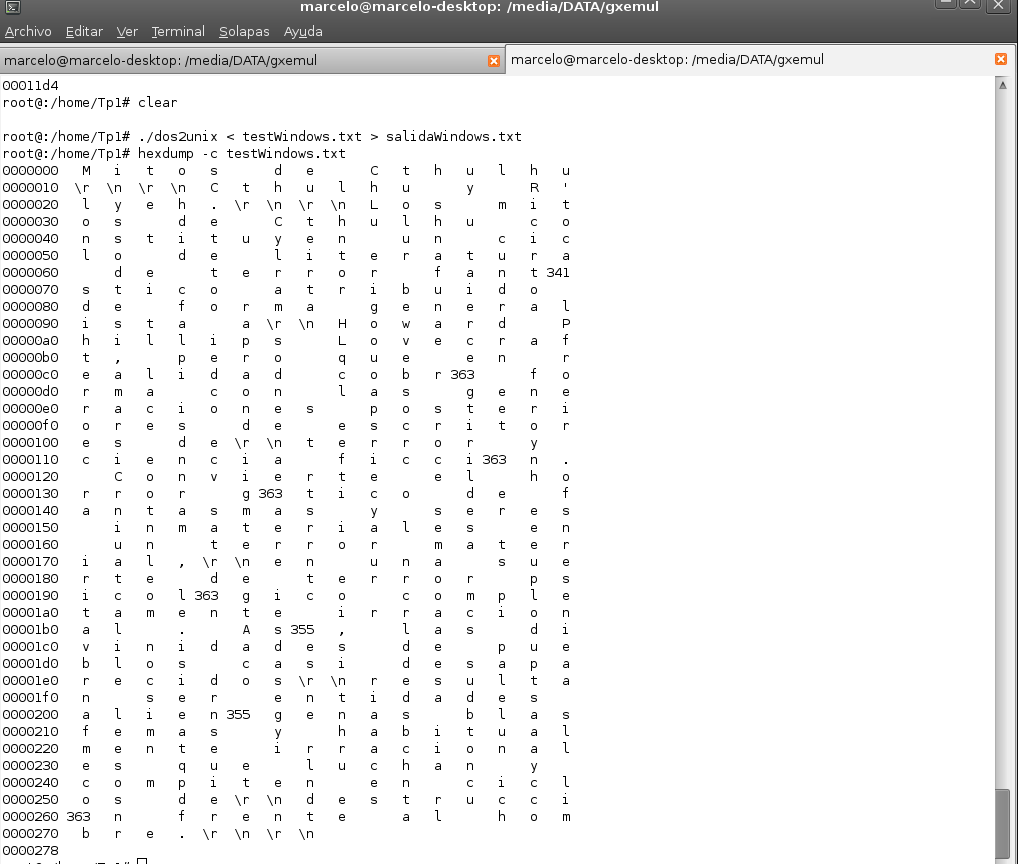
\includegraphics[width=10cm, viewport=0 0 1018 864]{Imagenes/testWindows.png}
     \newline
      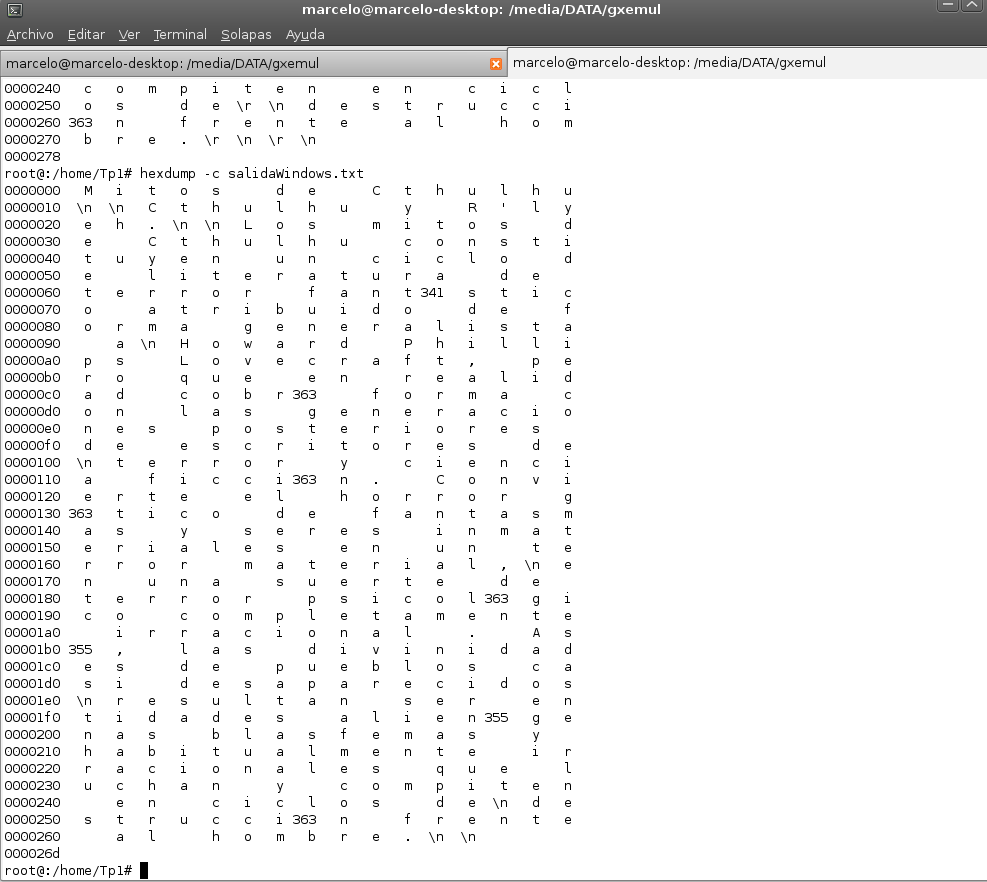
\includegraphics[width=10cm, viewport=0 0 987 882]{Imagenes/salidaWindows.png}
    \end{itemize}

\newpage
\section{Conclusiones}
  TODO

%APENDICES
\appendix
\newpage
\section{C\'odigo Fuente}
  \subsection{C\'odigo en C}
    \subsubsection{unix2dos.c}
      \lstset{numbers=left, frame=single, breaklines=true}
      \lstinputlisting{../src/CodigoC/unix2dos.c}
    \subsubsection{dos2unix.c}
      \lstset{numbers=left, frame=single, breaklines=true}
      \lstinputlisting{../src/CodigoC/dos2unix.c}
    \subsubsection{conversor.c}
      \lstset{numbers=left, frame=single, breaklines=true}
      \lstinputlisting{../src/CodigoC/conversor.c}
  \newpage
  \subsection{C\'odigo en Assembly}
    \subsubsection{unix2dos.S}
      \lstset{numbers=left, frame=single, breaklines=true}
      \lstinputlisting{../src/unix2dos.S}
    \subsubsection{dos2unix.S}
      \lstset{numbers=left, frame=single, breaklines=true}
      \lstinputlisting{../src/dos2unix.S}
    
\newpage
\section{Enunciado}
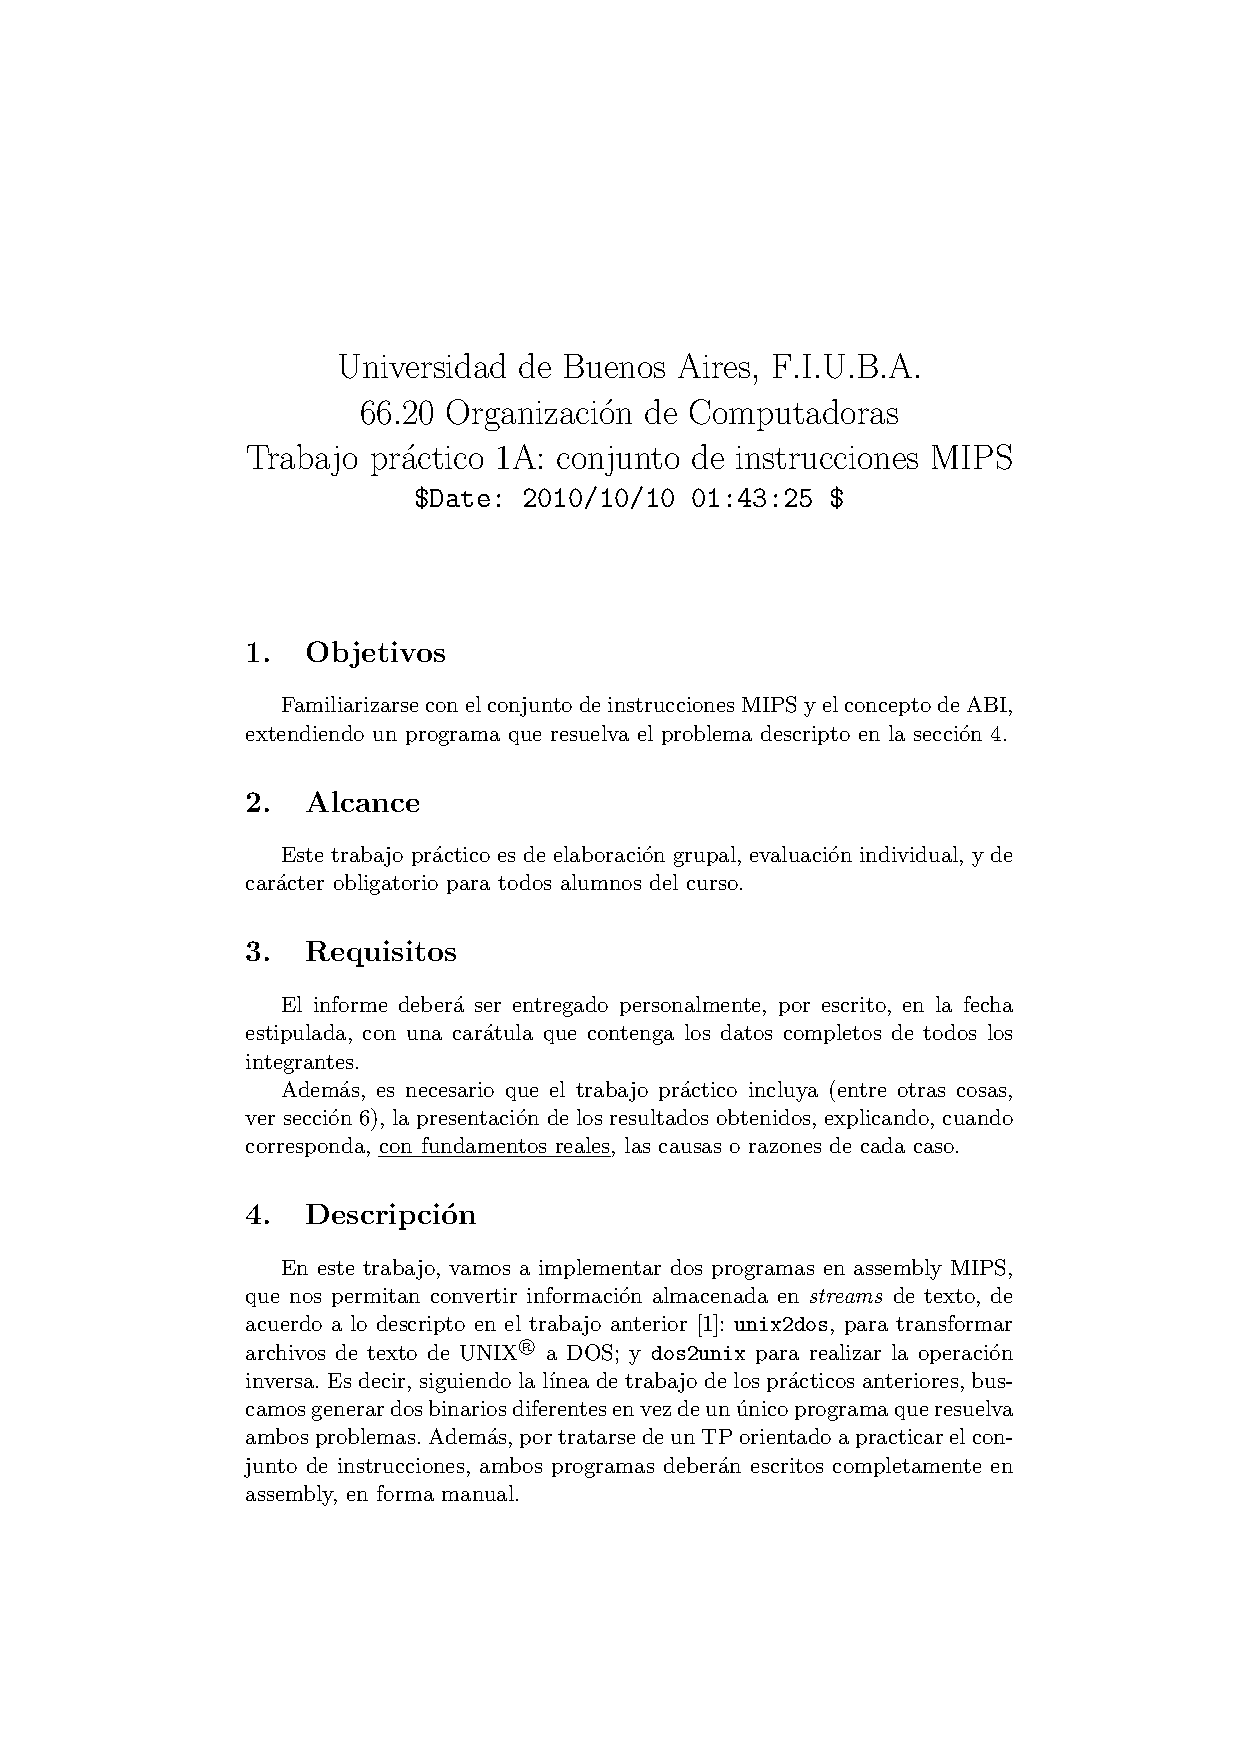
\includepdf[pages=1-3, scale=0.9, pagecommand={\thispagestyle{plain}}]{../tp1a-2010-2q.pdf}

\end{document}
